\documentclass[12pt,letterpaper]{exam}
\usepackage[lmargin=1in,rmargin=1in,tmargin=1in,bmargin=1in]{geometry}
\usepackage{../style/exams}

% -------------------
% Course & Exam Information
% -------------------
\newcommand{\course}{MAT 101: Exam 2}
\newcommand{\term}{Fall -- 2023}
\newcommand{\examdate}{11/08/2023}
\newcommand{\timelimit}{85 Minutes}

\setbool{hideans}{false} % Student: True; Instructor: False

% -------------------
% Content
% -------------------
\begin{document}

\examtitle
\instructions{Write your name on the appropriate line on the exam cover sheet. This exam contains \numpages\ pages (including this cover page) and \numquestions\ questions. Check that you have every page of the exam. Answer the questions in the spaces provided on the question sheets. Be sure to answer every part of each question and show all your work. If you run out of room for an answer, continue on the back of the page --- being sure to indicate the problem number.} 
\scores
\bottomline
\newpage

% ---------
% Questions
% ---------
\begin{questions}

% Question 1
\newpage
\question[10] Consider the relation $f$ shown below. 
	\[
	\fbox{
	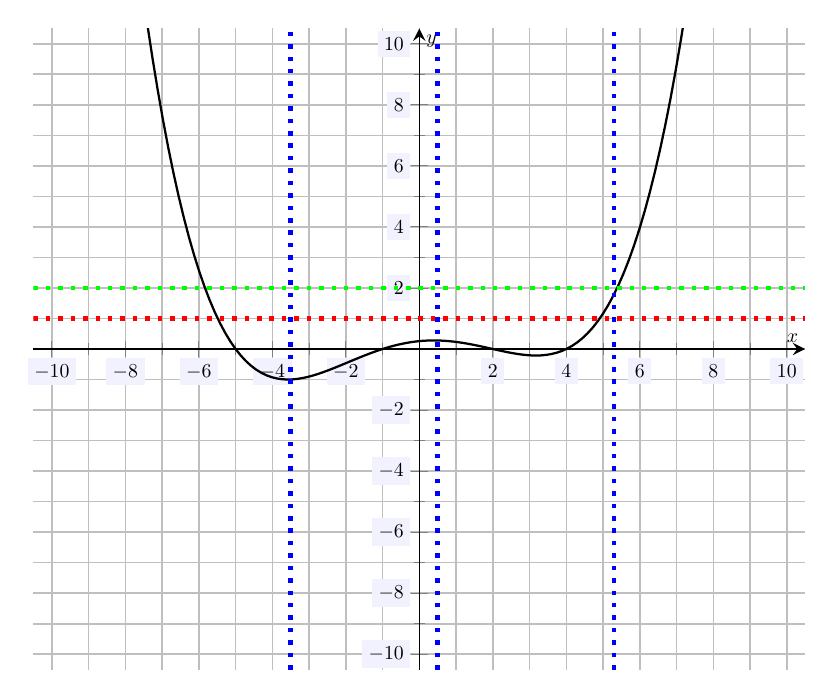
\begin{tikzpicture}[scale=1.43,every node/.style={scale=0.5}]
	\begin{axis}[
	grid=both,
	axis lines=middle,
	ticklabel style={fill=blue!5!white},
	xmin= -10.5, xmax=10.5,
	ymin= -10.5, ymax=10.5,
	xtick={-10,-8,-6,-4,-2,0,2,4,6,8,10},
	ytick={-10,-8,-6,-4,-2,0,2,4,6,8,10},
	minor tick = {-10,-9,...,10},
	xlabel=\(x\),ylabel=\(y\),
	]
	\addplot[line width= 0.02cm,samples=150,domain= -10.5:10.5] ({x},{1/155*(x - 4)*(x - 2)*(x + 1)*(x + 5)});
	
	\addplot[blue,dotted,line width= 0.04cm,samples=2,domain= -10.5:10.5] ({-3.5},{x});
	\addplot[blue,dotted,line width= 0.04cm,samples=2,domain= -10.5:10.5] ({0.5},{x});
	\addplot[blue,dotted,line width= 0.04cm,samples=2,domain= -10.5:10.5] ({5.3},{x});
	
	\addplot[red,dotted,line width= 0.04cm,samples=2,domain= -10.5:10.5] ({x},{1});
	
	\addplot[green,dotted,line width= 0.04cm,samples=2,domain= -10.5:10.5] ({x},{2});
	\end{axis}
	\end{tikzpicture}
	}
	\] 

\begin{enumerate}[(a)]
\item Is the relation shown above a function of $x$? Explain. 
\item Assuming the relation is a function of $x$, does the relation above have an inverse that is a function of $y$? Explain.
\item Find $f(6)$.
\item Find the $x$-intercepts of $f(x)$.
\item Is there an $x$ such that $f(x)= 2$? Explain. 
\end{enumerate} \pspace

\sol 
\begin{enumerate}[(a)]
\item Yes, the relation shown is a function because $f(x)$ passes the Vertical Line Test; that is, every vertical line intersects the graph of $f(x)$ at most once---some sample vertical lines are shown in blue. 

\item No, the relation shown does not have an inverse function $f^{-1}(x)$ because $f(x)$ fails the Horizontal Line Test; that is, not every horizontal line intersects the graph of $f(x)$ at most once. For instance, the horizontal line $y= 1$ (shown in red) intersects the graph of $f(x)$ twice, i.e. $f^{-1}(1)$ cannot be well defined. 

\item From the graph of $f(x)$, we can see that the graph contains the point $(6, 4)$, which implies $f(6)= 4$. 

\item The $x$-intercepts are the point(s) where the graph of $f(x)$ intersects the $x$-axis. From the graph of $f(x)$, we can see that these are $(-5, 0)$, $(-1, 0)$, $(2, 0)$, and $(4, 0)$, i.e. $x= -5, -1, 2, 4$. 
 
\item There are such $x$-values. If there is an $x$ such that $f(x)= 2$, then the line $y= 2$ (shown in green above) intersects the graph of $f(x)$. The $x$-value of such intersection points are $x$-values such that $f(x)= 2$. Examining the graph, we can see that if $x \approx -5.83284, 5.3828$, then $f(x)= 2$. 
\end{enumerate}



% Question 2
\newpage
\question[10] Consider invertible functions $f, g$, whose values at several specified $x$-values are given below. 
	\begin{table}[h]
	\centering
	\begin{tabular}{|c||c|c|c|c|c|} \hline
	$x$ & $-6$ & $2$ & $0$ & $5$ & $9$ \\ \hline
	$f$ & $1$ & $5$ & $2$ & $-6$ & $3$ \\ \hline
	$g$ & $0$ & $2$ & $9$ & $1$ & $6$ \\ \hline
	\end{tabular}
	\end{table}
Find the following:
	\begin{enumerate}[(a)]
	\item $(f + g)(9)$
	\item $(f \circ g)(0)$
	\item $\left( \frac{g}{f} \right)(2)$
	\item $y$-intercept of $f(x)$
	\item An $x$-intercept of $g(x)$
	\end{enumerate} \pspace

\sol 
\begin{enumerate}[(a)]
\item 
	\[
	(f + g)(9)= f(9) + g(9)= 3 + 6= 9
	\] \pspace

\item 
	\[
	(f \circ g)(0)= f \big( g(0) \big)= f(9)= 3
	\] \pspace

\item 
	\[
	\left( \dfrac{g}{f} \right)(2)= \dfrac{g(2)}{f(2)}= \dfrac{2}{5}
	\] \pspace

\item The $y$-intercept is the point/value where the graph of $f(x)$ intersects the $y$-axis. But this occurs when $x= 0$. So the $y$-intercept of $f(x)$ is the value $f(0)$:
	\[
	f(0)= 2
	\]
Therefore, the $y$-intercept of $f(x)$ is $(0, 2)$. \pspace

\item The $x$-intercept is the point(s)/value(s) where the graph of $g(x)$ intersects the $x$-axis. But this occurs when $g(x)= 0$. So the $x$-intercept(s) of $g(x)$ are the $x$-values for which $g(x)= 0$:
	\[
	g(-6)= 0
	\]
Therefore, the $x$-intercept of $g(x)$ is $(-6, 0)$. 
\end{enumerate}



% Question 3
\newpage
\question[10] Let $f(x)= x^2 + 2x - 1$, $g(x)= 3x + 8$, and $c$ be a constant. Showing all your work and simplifying as much as possible, compute the following:
	\begin{enumerate}[(a)]
	\item $(fg)(4)$
	\item $f(-2) - g(1)$
	\item $(f - g)(2)$
	\item $(f \circ g)(0)$
	\item $(g \circ f)(c)$
	\end{enumerate} \pspace

\sol First, observe that\dots
	\[
	\begin{aligned}
	f(-2)&= (-2)^2 + 2(-2) - 1= 4 - 4 - 1= -1 &\qquad g(0)&=  3(0) + 8= 0 + 8= 8 \\
	f(2)&= 2^2 + 2(2) - 1= 4 + 4 - 1= 7 & g(1)&= 3(1) + 8= 3 + 8= 11 \\
	f(4)&= 4^2 + 4(2) - 1= 16 + 8 - 1= 23 & g(2)&= 3(2) + 8= 6 + 8= 14 \\
	f(8)&= 8^2 + 2(8) - 1= 64 + 16 - 1= 79 & g(4)&= 3(4) + 8= 12 + 8= 20
	\end{aligned}
	\]
Then we have\dots
        \begin{enumerate}[(a)]
 	       \item 
    	    	\[
        		(fg)(4)= f(4) g(4)= 23 \cdot 20= 460
        		\] \pspace
        
        \item 
        		\[
        		f(-2) - g(1)= -1 - 11= -12
        		\] \pspace
        
        \item 
        		\[
        		(f - g)(2)= f(2) - g(2)= 7 - 14= -7
        		\] \pspace
        
        \item 
        		\[
        		(f \circ g)(0)= f \big( g(0) \big)= f(8)= 79
        		\] \pspace
        
        \item 
        		\[
        		(g \circ f)(c)= g \big( f(c) \big)= g(c^2 + 2c - 1)= 3(c^2 + 2c - 1) + 8= 3c^2 + 6c - 3 + 8= 3c^2 + 6c + 5
        		\]
        \end{enumerate}



% Question 4
\newpage
\question[10] Consider the function $\ell(x)= 4x - 6$.
	\begin{enumerate}[(a)]
	\item Is $\ell(x)$ linear? Explain. 
	\item Find the slope and $y$-intercept of $\ell(x)$. 
	\item Compute $\ell(\frac{17}{2})$. 
	\item Is there an $x$ such that $\ell(x)= 10$? Explain. 
	\item Find the $x$-intercept of $\ell(x)$. 
	\end{enumerate} \pspace

\sol 
\begin{enumerate}[(a)]
\item The function $\ell(x)= 4x - 6$ is linear because it has the form $y= mx + b$ with $y= \ell$, $x= x$, $m= 4$, and $b= -6$. \pspace

\item From (a), we have $m= 4$ and $b= -6$. Therefore, the slope is $m= 4$ and the $y$-intercept is $-6$, i.e. the point $(0, -6)$. \pspace

\item We have\dots
	\[
	\ell \left( \dfrac{17}{2} \right)= 4 \cdot \dfrac{17}{2} - 6= 2 \cdot 17 - 6= 34 - 6= 28
	\] \pspace

\item If there were such an $x$, we would have\dots
	\[
	\begin{gathered}
	\ell(x)= 10 \\
	4x - 6= 10 \\
	4x= 16 \\
	x= 4
	\end{gathered}
	\]
Finally, observe that $\ell(4)= 4(4) - 6= 16 - 6= 10$. Therefore, $x= 4$ is an $x$ such that $\ell(x)= 10$. \pspace

\item The $x$-intercept(s) of a function $f(x)$ are the $x$-values such that $f(x)= 0$. If $\ell(x)$ has an $x$-intercept, then $\ell(x)= 0$. But then\dots
	\[
	\begin{gathered}
	\ell(x)= 0 \\
	4x - 6= 0 \\
	4x= 6 \\
	x= \dfrac{6}{4} \\
	x= \dfrac{3}{2}
	\end{gathered}
	\]
Because $\ell(\frac{3}{2})= 4 \cdot \frac{3}{2} - 6= 2 \cdot 3 - 6= 6 - 6= 0$. Therefore, the $x$-intercept of $\ell(x)$ is $x= \frac{3}{2}$, i.e. the point $(\frac{3}{2}, 0)$. 
\end{enumerate}



% Question 5
\newpage
\question[10] Find the equation of the line that has $y$-intercept 5 that is parallel to the line shown below. 
	\[
	\fbox{
	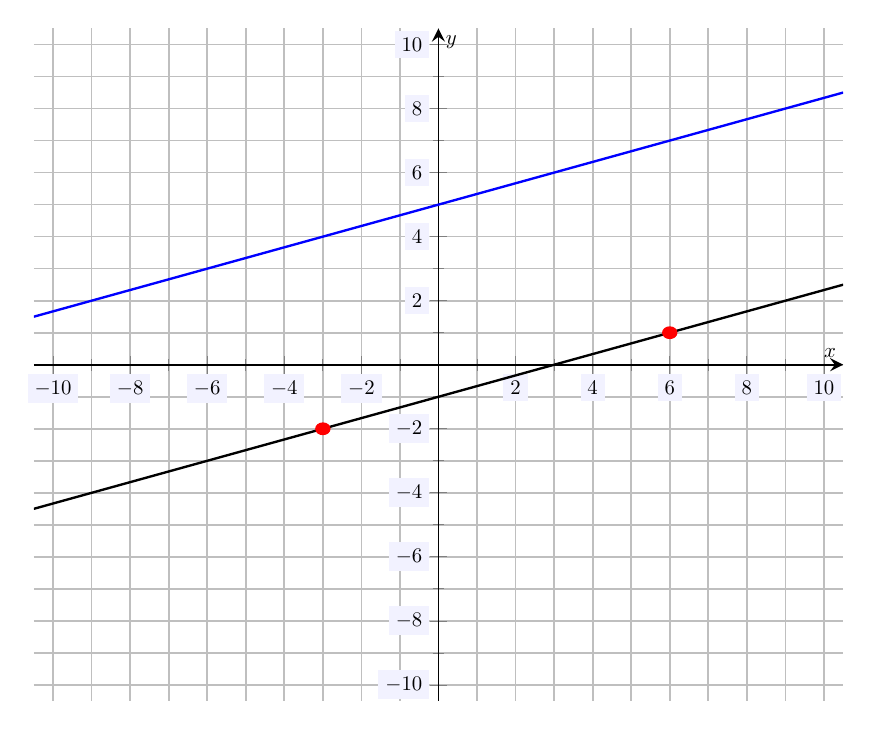
\begin{tikzpicture}[scale=1.5,every node/.style={scale=0.5}]
	\begin{axis}[
	grid=both,
	axis lines=middle,
	ticklabel style={fill=blue!5!white},
	xmin= -10.5, xmax=10.5,
	ymin= -10.5, ymax=10.5,
	xtick={-10,-8,-6,-4,-2,0,2,4,6,8,10},
	ytick={-10,-8,-6,-4,-2,0,2,4,6,8,10},
	minor tick = {-10,-9,...,10},
	xlabel=\(x\),ylabel=\(y\),
	]
	\addplot[line width= 0.02cm,samples=50,domain= -10.5:10.5] ({x},{1/3*x - 1});
	\addplot[blue,line width= 0.02cm,samples=50,domain= -10.5:10.5] ({x},{1/3*x + 5});
	
	\draw[fill=red,draw=none] (-3,-2) circle (0.2);
	\draw[fill=red,draw=none] (6,1) circle (0.2);
	\end{axis}
	\end{tikzpicture}
	}
	\] \pspace

\sol Because the given line is not vertical, any line parallel to this line will also not be vertical. Then the line in question must have the form $y= mx + b$ for some $m, b$. Because the line in question is parallel to the line shown, it must have the same slope as the given line. Using the points in red on the given line, we compute the slope of the line shown above:
	\[
	m= \dfrac{\Delta y}{\Delta x}= \dfrac{1 - (-2)}{6 - (-3)}= \dfrac{1 + 2}{6 + 3}= \dfrac{3}{9}= \dfrac{1}{3}
	\]
But then we have $y= \frac{1}{3}\,x + b$. Because $b$ is the $y$-intercept and the line in question must have $y$-intercept 5, we must have $y= \frac{1}{3}\,x + 5$. We plot this line in blue on the plot above. 



% Question 6
\newpage
\question[10] Find the equation of the line with $x$-intercept $-6$ that passes through the point of intersection of $y= 5x - 1$ and $y= 6 - 2x$. \pspace

\sol We know the line in question has $x$-intercept $-6$, i.e. the graph of the line contains the point $(-6, 0)$. We know the line in question also contains the point of intersection of $y= 5x - 1$ and $y= 6 - 2x$. But at this point of intersection, the lines have the same $x$ and $y$-value. But then\dots
	\[
	\begin{gathered}
	y= y \\
	5x - 1= 6 - 2x \\
	7x - 1= 6 \\
	7x= 7 \\
	x= 1
	\end{gathered}
	\]
But then $y(1)= 5(1) - 1= 5 - 1= 4$ (or $y(1)= 6 - 2(1)= 6 - 2= 4$). Therefore, the line in question also contains the point $(1, 4)$. Because $1 \neq -6$, we know the line in question is not vertical; therefore, it must have the form $y= mx + b$ for some $m, b$. Using the points $(-6, 0)$ and $(1, 4)$, we can compute the slope of the line in question:
	\[
	m= \dfrac{\Delta y}{\Delta x}= \dfrac{4 - 0}{1 - (-6)}= \dfrac{4 - 0}{1 + 6}= \dfrac{4}{7}
	\]
We then have $y= \frac{4}{7}\,x + b$. Because the line contains the point $(-6, 0)$, when $x= -6$, $y= 0$. But then\dots
	\[
	\begin{gathered}
	y= \dfrac{4}{7}\,x + b \\[0.3cm]
	0= \dfrac{4}{7} \cdot -6 + b \\[0.3cm]
	0= -\dfrac{24}{7} + b \\[0.3cm]
	b= \dfrac{24}{7}
	\end{gathered}
	\] \pspace
Therefore, $y= \frac{4}{7}\,x + \frac{24}{7}= \frac{4x + 24}{7}= \frac{4(x + 6)}{7}$.



% Question 7
\newpage
\question[10] Consider the lines $\ell_1(x)= 6x - 17$ and $\ell_2(x)= 8 - 11x$. 
	\begin{enumerate}[(a)]
	\item Determine whether the given lines are parallel, perpendicular, or neither. Justify your answer.
	\item Do the lines intersect? If not, explain why. If so, find their point of intersection. 
	\end{enumerate} \pspace

\sol 
\begin{enumerate}[(a)]
\item The slope of $\ell_1(x)= 6x - 17$ is $m_1= 6$. The slope of $\ell_2(x)= 8 - 11x$ is $m_2= -11$. Because $m_1 \neq m_2$, the lines are not parallel. Furthermore, because $m_1= 6 \neq \frac{1}{11}= -\frac{1}{m_2}$, the lines are not perpendicular. Therefore, $\ell_1$ and $\ell_2$ are neither parallel nor perpendicular. \pspace

\item Because $\ell_1$ and $\ell_2$ are not parallel, they intersect. At their point of intersection, the lines have the same output for the same input. But then\dots
	\[
	\begin{gathered}
	\ell_1(x)= \ell_2(x) \\
	6x - 17= 8 - 11x \\
	17x - 17= 8 \\
	17x= 25 \\
	x= \dfrac{25}{17}
	\end{gathered}
	\]
But then\dots
	\[
	\begin{aligned}
	\ell_1 \left( \dfrac{25}{17} \right)&= 6 \cdot \dfrac{25}{17} - 17= \dfrac{150}{17} - 17= \dfrac{150}{17} - \dfrac{289}{17}= -\dfrac{139}{17} \\[0.3cm]
	\ell_2 \left( \dfrac{25}{17} \right)&= 8 - 11 \cdot \dfrac{25}{17}= 8 - \dfrac{275}{17}= \dfrac{136}{17} - \dfrac{275}{17}= -\dfrac{139}{17}
	\end{aligned}
	\]
Therefore, $\ell_1(x)$ and $\ell_2(x)$ intersect at the point $\left( \dfrac{25}{17}, -\dfrac{139}{17} \right)$. 
\end{enumerate}



% Question 8
\newpage
\question[10] Consider the function given by $f(x)= 11 - 9x$.
	\begin{enumerate}[(a)]
	\item Explain why $f^{-1}(x)$ exists. 
	\item Find $f^{-1}(x)$.
	\item Use $f^{-1}$ to solve the equation $f(x)= \frac{17}{9}$. 
	\end{enumerate} \pspace

\sol 
\begin{enumerate}[(a)]
\item The function $f(x)= 11 - 9x$ is a linear function because it has the form $y= mx + b$, where $y= f$, $x= x$, $m= -9$, and $b= 11$. Because $f(x)$ is not a vertical line, it must pass the Horizontal Line Test. Therefore, $f^{-1}(x)$ must exist. \pspace

\item We interchange the role of $y= f(x)$ and $x$ and solve for $y$ to find $f^{-1}(x)$. Interchanging the variables, we have $y= 11 - 9x \squiggle x= 11 - 9y$. But then\dots
	\[
	\begin{gathered}
	x= 11 - 9y \\
	x - 11= -9y \\
	y= \dfrac{x - 11}{-9} \\
	y= \dfrac{11 - x}{9}
	\end{gathered}
	\]
Therefore, $f^{-1}(x)= \frac{11 - x}{9}$. One can confirm this: $f^{-1}(f(x))= f^{-1}(11 - 9)= \frac{11 - (11 - 9x)}{9}= \frac{9x}{9}= x$ and $f(f^{-1}(x))= f(\frac{11 - x}{9})= 11 - 9(\frac{11 - x}{9})= 11 - (11 - x)= x$. \pspace

\item We have\dots
	\[
	\begin{gathered}
	f(x)= \dfrac{17}{9} \\[0.2cm]
	f^{-1} \big( f(x) \big)= f^{-1} \left( \dfrac{17}{9} \right) \\[0.2cm]
	x= \dfrac{11 - x}{9} \bigg|_{x= \frac{17}{9}} \\[0.2cm]
	x= \dfrac{11 - \frac{17}{9}}{9} \\[0.2cm]
	x= \dfrac{\frac{82}{9}}{9} \\[0.2cm]
	x= \dfrac{82}{81}
	\end{gathered}
	\]
\end{enumerate}



% Question 9
\newpage
\question[10] An \textit{arithmetic sequence} is a list of numbers where the difference between one number and the next is always the same. For instance, 2, 6, 10, 14, 18, \dots is an arithmetic sequence because the difference between sequential terms is always 4, while the sequence 1, 2, 3, 5, 7, 10, 13, \dots is \textit{not} an arithmetic sequence because the difference between sequential terms is not constant. Let $S$ be the sequence 34, 57, 80, 103, 126, \dots. 
	\begin{enumerate}[(a)]
	\item Find a function $S(n)$ that gives the $n$th term of the sequence. 
	\item Find the 835th term of the sequence. 
	\item Is 3,500 a term of this sequence? Explain. 
	\end{enumerate} \pspace

\sol Observe that the sequence $S$ is arithmetic because $23= 57 - 34= 80 - 57= 103 - 80= 127 - 103= \cdots$. 

\begin{enumerate}[(a)]
\item Because the terms of the sequence change by a constant rate, we can represent the $n$th term of the sequence by a linear function. Let $S(n)$ denote the $n$th term of the sequence. Then we know $S(n)= mn + b$. Because each term of the sequence is 23 more than the last, we know that $m= 23$. But then $S(n)= 23n + b$. We know that $S(1)= 34$. But $34= S(1)= 23(1) + b= 23 + b$. So $b + 23= 34$, which implies $b= 11$. Therefore, $S(n)= 23n + 11$. \pspace

\item This is $S(835)$. But we have\dots
	\[
	S(835)= 23(835) + 11= 19205 + 11= 19216
	\] \pspace

\item Every term of the sequence is of the form $S(n)= 3500$. If 3500 were a term of the sequence, then there would be a whole number $n$ such that $S(n)= 3500$. But then\dots
	\[
	\begin{gathered}
	S(n)= 3500 \\
	23n + 11= 3500 \\
	23n= 3489 \\
	n= 151.696
	\end{gathered}
	\]
Because $n$ is not a whole number, 3,500 cannot be a term of the sequence. 
\end{enumerate}



% Question 10
\newpage
\question[10] A cleaning service does not have their prices listed on their website but the site does mention they charge a fixed amount per hour. You make some calls and have one friend that used their service and paid \$212.50 for a 3~hour cleaning while another friend paid \$400 for a 6~hour cleaning. Let $C(h)$ be the cost the service will charge for $h$~hours of cleaning.
	\begin{enumerate}[(a)]
	\item Explain why $C(h)$ is linear.
	\item Find $C(h)$.
	\item Interpret the slope and $y$-intercept for $C(h)$.
	\item How many hours of cleaning can you get for \$950?
	\end{enumerate} 

\sol 
\begin{enumerate}[(a)]
\item Because the cost of the cleaning increases at a constant rate per hour, $C(h)$ must be a linear function. 

\item From (a), we know that $C(h)$ is linear. Then $C(h)= mh + b$ for some $m, b$. We know that a 3~hour cleaning costs \$212.50 and a 6~hour cleaning costs \$400, i.e. $(3, 212.50)$ and $(6, 400)$ are points on the graph of $C(h)$. But then\dots
	\[
	m= \dfrac{\Delta C}{\Delta h}= \dfrac{400 - 212.50}{6 - 3}= \dfrac{187.50}{3}= 62.5
	\]
Thus, $C(h)= 62.5h + b$. Using the fact that $(6, 400)$ on the graph of $C(h)$, we know $C= 400$ when $h= 6$. But then\dots
	\[
	\begin{gathered}
	C(h)= 62.5h + b \\
	C(6)= 62.5(6) + b \\
	400= 375 + b \\
	b= 25
	\end{gathered}
	\]
Therefore, $C(h)= 62.5h + 25$. \pspace

\item The slope of $C(h)$ is $m= 62.50$. Because $m= \frac{\Delta C}{\Delta h}$, we know that $m= \$62.50/\text{hr}$. But then we know every additional hour of cleaning increases the price charged by \$62.50, i.e. the service charges \$62.50 per hour. The $y$-intercept of $C(h)$ is $b= 25$. This is the cost of cleaning for $h= 0$~hours of cleaning. This must represent some type of service, processing, arrival, etc. charge for the cleaning. This could also represent a minimal charge. \pspace

\item If $h_0$ is the number of hours of cleaning one can get for \$950, then $C(h_0)= 950$. But then\dots
	\[
	\begin{gathered}
	C(h_0)= 950 \\
	62.5h_0 + 25= 950 \\
	62.5h_0= 925 \\
	h_0 \approx 14.8
	\end{gathered}
	\]
Therefore, one can receive up to 14.8~hours of cleaning for \$950. 
\end{enumerate}


\end{questions}
\end{document}